\documentclass{standalone}
\usepackage{amsmath}
\usepackage{amsfonts}
\usepackage{tikz}
\usetikzlibrary{arrows,shapes,positioning,shadows,trees}

\begin{document}
\begin{tikzpicture}
    \draw[-] (0,0) -- (0,0) node[anchor=center] {$\times$};
    \draw [->] plot [smooth, tension=1, circle] coordinates {(1.75,0) (1,1.5) (0,1) (-2,0.5) (0,-1) (1.5,-0.8) (1.75,0)};
    \node[above right] at (1.75,0) {$\gamma$};
\end{tikzpicture}
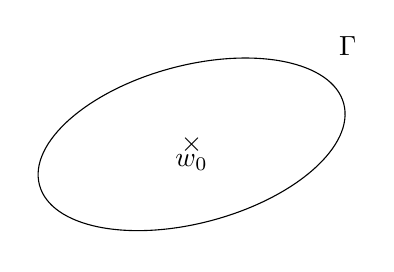
\begin{tikzpicture}
    \draw[-] (0,0) -- (0,0) node[anchor=center] {$\times$};
    \node[below] at (0,0) {$w_0$};
    \draw (0,0) [rotate=15] ellipse (2cm and 1cm);
    \node[above right] at (1.75,1) {$\Gamma$};
\end{tikzpicture}
\end{document}